\section{Experimental Evaluation}
\label{sec:exps}
In this section we present an empirical evaluation of our proposed algorithmic framework. The main questions we seek to address are: (1) how the proposed querying policy algorithm compares against baselines for maximizing the number of extracted entities under a specific budget, (2) how the different gain estimators presented in \Cref{sec:gainestimators} compare with each other, and (3) how the proposed querying policy algorithm exploits the structure of the input domain to construct the set of available actions.

We empirically study these questions using both real and synthetic datasets. First, we discuss the experimental methodology, and then we describe the data and results that demonstrate the effectiveness of our framework on crowdsourced entity extraction. The evaluation is performed on an Inter(R) Cored(TM) i7 3.7 GHz/64bit/32GB machine. The proposed framework is implemented in Python 2.7. 

\vspace{5pt}\noindent\textbf{Gain Estimators:} We evaluate the following gain estimators:
\squishlist
\item Chao92Shen: This estimator combines the methodology proposed by Chao~\cite{chao:1992} for estimating the number of unseen species  with Shen's formula~\Cref{eq:shen}. This approach has been used by Trushkowsky et al.~\cite{trushkowsky:2013} in their evaluation.
\item HwangShen: This estimator combines the regression based approach proposed by Hwang and Shen~\cite{hwang:2010} for estimating the number of unseen species with Shen's formula. 
\item NewRegr: This estimator corresponds to the new regression based technique proposed in \Cref{sec:newestim}.
\squishend
All estimators were coupled with bootstrapping to estimate their variance. Computing the variance of each estimator is required to retrieve an upper bound on the return of a query as shown in \Cref{eq:upper}.

\vspace{5pt}\noindent\textbf{Entity Extraction Algorithms:} We evaluate the following algorithms for crowdsourced entity extraction:
\squishlist
\item Rand: This algorithm executes random queries over the input domain until all the available budget is used. It selects a random node from the input poset $\hierarchy$ and a random query configuration $q(k,l)$ from a list of pre-specified $k$, $l$ value combinations. We expect Rand to be effective for extracting entities in small and dense data domains that do not have a large number of sparsely populated nodes. 
\item RandL: This algorithm executes random queries {\em only at the lowest level nodes} (i.e., leaf nodes) of the input poset $\hierarchy$ until all the available budget is used. It selects a random node and a random query configuration $q(k,l)$ from a list of pre-specified $k$, $l$ value combinations. Similarly to Rand we expect RandL to be effective for {\em shallow} hierarchies when the majority of nodes corresponds to leaf nodes. Again the performance of RandL is expected to be reasonable for small and dense data domains without sparsely populated nodes. 
\item BFS: This algorithm performs a breadth-first traversal of the input poset $\hierarchy$. It only executes {\em one query} at a given node. The query configuration is randomly selected from a list of pre-specified $k$, $l$ value combinations. This algorithm promotes exploration of the action space when extracting entities. It also takes into account the structure of the input domain but is agnostic to sparsely populated areas of the domain.
\item GSChao: This algorithm corresponds to our proposed heuristic shown in \Cref{sec:heuristic} and uses the Chao92Shen estimator to estimate the gain of additional queries.
\item GSHwang: This algorithm corresponds to our proposed heuristic shown in \Cref{sec:heuristic} and uses the HwangShen estimator to estimate the gain of additional queries.
\item GSNewR: This algorithm corresponds to our proposed heuristic shown in \Cref{sec:heuristic} and uses the NewRegr estimator to estimate the gain of additional queries.
\item GSExact: This algorithm is used as a near-optimal baseline. In particular, we combine the heuristic proposed in \Cref{sec:heuristic} with an exact computation of the query return. More precisely, the algorithm proceeds as follows: At each round we speculatively execute each of the available actions and select the one that results in the largest  number of return to cost ratio. Since the return of each query is known, the algorithm is not coupled with any of the aforementioned estimators.
\squishend
We run each algorithm multiple times as the results of each run depend on the sampled entities front the underlying unknown population. For each algorithm we report the average gain achieved under the given budget as well as the corresponding standard errors.

\vspace{5pt}\noindent\textbf{Querying Interface:} For all datasets we consider generalized queries $q(k,l)$ of the type ``Give me $k$ more entities that satisfy a set of predicates and are not present in an exclude list of size $l$". The specified predicates correspond to the attribute values associated with a node from the input poset. The  configurations considered for $(k,l)$ are $\{(5,0), (10,0), (20,0), (5,2), (10,5), (20,5), (20,10)\}$. Larger values of $k$ or $l$ were deemed unreasonable for crowdsourced queries. The gain of a query is computed as the number of new entities extracted. The cost of each query is computed using an additive model comprised by three partial cost terms that depend on the characteristics of the query. 

The three partial cost terms are: (i) {\sf CostK} that depends on the number of responses $k$ requested from a user, (ii) {\sf CostL} that depends on the size of the exclude list $l$ used in the query, and (iii) {\sf CostSpec} that depends on the {\em specificity} of the query $q_s$, e.g., we assume that queries that require users to provide more specialized entities such as a ``Give me one concert for New York on the 17th of Nov" cost more than more generic queries such as ``Give me one concert in New York". More formally, we define the specificity of a query to be equal to the number on attributes assigned non-wildcard values for the node $u \in \hierarchy$ the query corresponds to. 

For each of the cost terms we assume a maximum cost of \$1 realized by considering the maximum value of the corresponding input variable. More precisely, we have that:
\begin{align}
{\sf CostK}(k^{\prime}) &= \frac{k^{\prime}}{\mbox{max. $k$ value}} \nonumber \\
{\sf CostL}(l^{\prime}) &= \frac{l^{\prime}}{\mbox{max. $l$ value}} \nonumber \\
{\sf CostSpec}(q_{s^{\prime}}) &= \frac{s^{\prime}}{\mbox{max. specificity value}} \nonumber
\end{align}
The overall cost for a query is then computed as:
\begin{equation}
Cost(q(k,l)) = \alpha \cdot {\sf CostK}(k) + \beta \cdot  {\sf CostK}(k) + \gamma \cdot  {\sf CostSpec}(q_s) \nonumber
\end{equation}
Since the cost of a query should be significantly increased when an exclude list is used we set $\alpha = \gamma = 1$ and $\beta = 5$. 

\subsection{Synthetic Data Experiments}
\label{sec:synthetic}
First, we evaluate the proposed framework on extracting entities from a large domain. We consider the event dataset collected from Eventbrite. As described in \Cref{sec:intro} the lattice corresponding to the Eventbrite domain contains 8,508,160 points with 57,805 distinct events overall. However, only 175,068 points are populated leading to an rather sparsely populated domain. Due to luck of popularity proxies for the extracted events, we assigned a random {\em popularity weight} in $(0,10]$ to each event. These weights are used during sampling to form the actual popularity distribution characterizing the population of each point in the lattice. 

\noindent\textbf{Results:} First, we evaluate the performance of the gain estimators described above at predicting the number of new retrieved events for different query configurations. We choose ten random points from the Eventbrite lattice each containing more than 5,000 events . For each of the points and each of the available query parameter configurations $(k,l)$, we execute ten queries of the form ``Give me $k$ items from point $u \in \hierarchy$ that are not included in an exclude list of size $l$". As mentioned in \Cref{sec:excludelist} the exclude list for each query is constructed following a randomized approach. We evaluate the performance of Chao92Shen, HwangShen, and NewRegr at predicting the return of each query. We measure the performance of each estimator by considering the absolute relative error between the predicted return and the actual return of the query. In \Cref{tab:eventesterror} we report the relative error for each of the three estimators averaged over all points under consideration. As shown, all three estimators perform equivalently with the new regression based technique slightly outperforming Chao92Shen and HwangShen for certain types of queries. The increased number of relative errors are justified as the retrieved samples correspond to a very small portion of the underlying population for each of the points. This is a well-known behavior for non-parametric estimators and studied extensively in the species estimation literature~\cite{hwang:2010}. 

\begin{table}
\small\center
\caption{Average absolute relative error for estimating the gain of different generalized queries. The results reported correspond to the average error over multiple queries issued at multiple points of the Eventbrite lattice.}
\label{tab:eventesterror}
\begin{tabular}{|c|c|c|c|c|}
\hline
\textbf{Q. Size $k$} & \textbf{EL. Size $l$} & \textbf{Chao92Shen} & \textbf{HwangShen} & \textbf{NewRegr} \\ \hline
5 & 0 & 0.470 & 0.500 & 0.427 \\
5 & 2 & 0.554 & 0.612 & 0.567\\
10 & 0 & 0.569 & 0.592 & 0.544\\
10 & 5 & 0.580 & 0.696 & 0.559\\
20 & 0 & 0.642 & 0.756 &0.601\\
20 & 5 & 0.510 & 0.60 & 0.519 \\
20 & 10 & 0.653 & 0.756 & 0.631\\
\hline
\end{tabular}
\vspace{-10pt}
\end{table}


Next, we evaluate the performance of our proposed algorithmic framework when extracting events from the Eventbrite domain. We evaluate the performance of the different extraction algorithms described above for different budgets. We ran each algorithm ten times and report the average number of unique events extracted as well as the corresponding standard error. The results are shown in \Cref{fig:ebextraction}. As shown all of our proposed algorithms, i.e., GSChao, GSHwang, GSNewR outperform the baselines under consideration exhibiting an improvement of at least 2x on the total number of unique events extracted. Moreover, for smaller budgets we observe that these algorithms perform comparably to GSExact that has oracle access to the gain of each query.

\begin{figure}[h]
	\begin{center}
	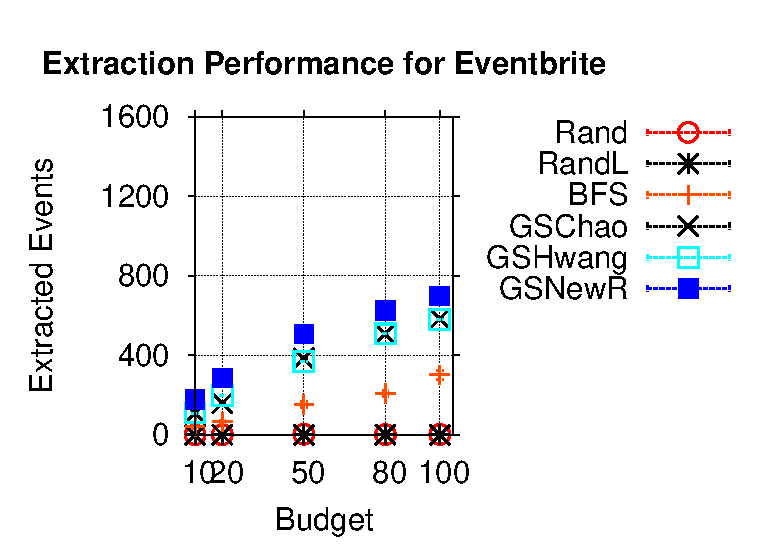
\includegraphics[clip,scale=0.6]{figs/ebExtraction.eps}
	\caption{The number of events extracted by different algorithms for the Eventbrite data domain and different budgets.}
	\label{fig:ebextraction}
	\end{center}
\end{figure}

The poor performance of Rand and RandL is due to the sparsity of the Eventbrite data domain. Regarding BFS, we see that it exhibits better performance than Rand and RandL by exploiting the structure of the underlying domain. However, since BFS is agnostic to the cost of the issued queries as well as to sparsely populated areas of the underlying lattice it can only extract a limited number of events. On the other hand, our proposed techniques were able to extract significantly more tuples as they both exploit the structure of the lattice and optimize for the cost of the issued queries. Finally, we point out that GSNewR that combines the proposed lattice traversal heuristic with our new regression-based gain estimator was able to outperform GSChao and GSHwang which rely on well-known estimators from the species estimation literature. This improved performance stems from the fact that our regression-based technique is capable of deriving better gain estimates in the presence of very small smalls and queries where workers are requested to provide a small number of answers.


\subsection{Real Data Experiments}
\label{sec:realdata}
Since the performance of the baselines algorithms is significantly affected by the sparsity of the Eventbrite domain, we chose to further evaluate the performance of the extraction algorithms listed above for a smaller, thus more dense domain. For this purpose, we use a real-world dataset collected via Amazon Mechanical Turk~\cite{mturk}. 

We asked workers to extract the names of people belonging in four different types from five different news portals. The people types we considered were ``Politicians", ``Athletes", ``Actors/Singers" and ``Industry People". The news portals we considered were ``New York Times", ``Huffington Post", ``Washington Post", ``USA  Today" and ``The Wall Street Journal". The domain under consideration is specified by the two attributes corresponding to the type of the person and the news portal. The lattice corresponding to this domain was constructed by taking the crossproduct of the aforementioned values. Workers were paid \$0.20 per HIT to provide items belonging in the specified data domain. We issued 20 HITS for each leaf node of the lattice, resulting in 600 HITS in total and extracted 1,245 people in total. \Cref{tab:ptypedata} and \Cref{tab:ntypedata} show the number of distinct entities for the different values of the people-type and news portal attributes. Finally, the popularity weight of each extracted entity was assigned to be equal to the number of times it appeared in the extraction result. These weights are then normalized during sampling time to form a proper popularity distribution.

\begin{table}
\center
\caption{The population characteristics of the AMT data.}
\label{tab:ptypedata}
\begin{tabular}{|c|c|}
\hline
\textbf{Person Type} & \textbf{People} \\ \hline
Industry People & 743 \\
Athletes & 743 \\
Politicians & 748 \\
Actors/Singers & 744 \\ \hline \hline
\end{tabular}
\end{table}


\begin{table}
\center
\caption{The population characteristics of the AMT data.}
\label{tab:ntypedata}
\begin{tabular}{|c|c|}
\hline
\textbf{News Portal} & \textbf{People} \\ \hline
WSJ & 594 \\
WashPost & 597 \\
NY Times & 595 \\
HuffPost & 599 \\
USA Today & 593 \\ \hline
\end{tabular}
\end{table}


\noindent\textbf{Results}: We first evaluate the performance of the gain estimators. As before, we issue ten generalized queries to different nodes of the input lattice for all available query configurations. Since the input domain is rather small we issued ten queries over all nodes in the input lattice. For each gain estimator and query configuration, we computed the average relative error, comparing the estimated query return with the actual query return. The results are shown in \Cref{tab:peopleesterror}. Again, we observe that for smaller query sizes the regression techniques proposed in this paper offers better gain estimates. However, as the query size increases, and hence, a larger portion of the underlying population is observed we see that Chao92Shen outperforms both regression based techniques. 

\begin{table}
\small\center
\caption{Average absolute percentage error for estimating the gain of different generalized queries. The results reported correspond to  averaged over multiple queries issued at all points of the People data domain.}
\label{tab:peopleesterror}
\begin{tabular}{|c|c|c|c|c|}
\hline
\textbf{Q. Size $k$} & \textbf{EL. Size $l$} & \textbf{Chao92Shen} & \textbf{HwangShen} & \textbf{NewRegr} \\ \hline
5 & 0 & 0.295 & 0.299 & 0.228\\
5 & 2 & 0.163 &  0.156 & 0.144\\
10 & 0 &  0.306 & 0.305 & 0.277\\
10 & 5 &  0.341 & 0.349 & 0.293\\
20 & 0 &  0.359& 0.371 & 0.467 \\
20 & 5 &  0.402 & 0.418 & 0.493\\
20 & 10 & 0.405 & 0.428 & 0.638\\
\hline
\end{tabular}
\vspace{-10pt}
\end{table}

Finally, we evaluate the performance of the different extraction algorithms. Similarly to Eventbrite we ran each algorithm ten times and report the average performance and the corresponding standard error. The results are shown in \Cref{fig:poextraction}. As shown our proposed techniques (i.e., GSChao, GSHwang and GSNewR) still outperform Rand, RandL and BFS. However, we see that the performance improvement is smaller compared to Eventbrite. The reason is that the people's domain is dense and all nodes of the input lattice are populated. 

\vspace{-10pt}\begin{figure}[h]
	\begin{center}
	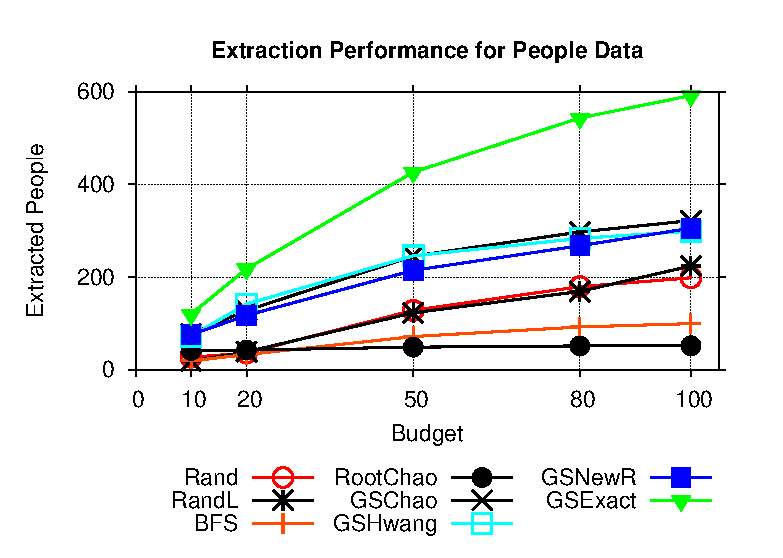
\includegraphics[clip,scale=0.6]{figs/poExtraction.eps}
	\caption{The number of people extracted by different algorithms for the People data domain and different budgets.}
	\label{fig:poextraction}
	\end{center}
	\vspace{-10pt}
\end{figure}

In particular, we observe that issuing random extraction queries at the nodes of the lattice outperforms BFS for a significant margin as the available budget increases. This behavior is expected in dense small domains where all the available nodes are populated. Notice that this approach corresponds to a querying policy that focuses purely on exploring different queries. However, exploited previously obtained information and balancing exploration and exploitation of the possible actions (i.e., following the proposed lattice traversal algorithm) leads to superior performance. 


\subsection{Take-Away Points}
We have the following recommendations according to the experimental results.
\squishlist
\item Exploiting the structure of the entity extraction domain is effective for maximizing the total number of extracted entities. Moreover, balancing the exploration of queries for non-observed nodes of the lattice with queries over observed nodes of the lattice is crucial.
\item For sparse domains, i.e., domain specified by large lattices with a small number of populated nodes, one should resolve to regression based techniques for estimating the expected gain of further queries as they result in better performance. However, for dense domains the Chao92Shen estimator results in better performance as a larger portion of the underlying population can be sampled. The size of the input domain as well as its sparsity are known in advance to the designed of the querying interface. 
\item For small budgets the proposed estimator-based lattice traversal algorithms (i.e., GSChao, GSHwang and GSNewR) exhibit comparable performance with a traversal algorithm that has oracle access to the gain of each query to be issued.
\squishend